\documentclass{chi-ext}
\usepackage[T1]{fontenc}
\usepackage[utf8]{inputenc}
\usepackage{lmodern}

% Please be sure that you have the dependencies (i.e., additional LaTeX packages) to compile this example.
% See http://personales.upv.es/luileito/chiext/

\copyrightinfo{
  Copyright is held by the author/owner(s).\\
  This is a generic SIGCHI \LaTeX\ template sample.\\
  The corresponding ACM copyright statement must be included.
}

\title{HCI-Projektbericht Draw-to-Clipboard}

\numberofauthors{8}
% Notice how author names are alternately typesetted to appear ordered in 2-column format;
% i.e., the first 4 autors on the first column and the other 4 auhors on the second column.
% Actually, it's up to you to strictly adhere to this author notation.
\author{
  \vspace{-1.5em} % lisatolles: The abstract heading should start at the time height on the page as the authors names
  \alignauthor{
  	\textbf{Marcus Vetter}\\
  	\email{marcus.vetter@tum.de}
  }
  \vfil
  \alignauthor{
  	\textbf{Constantin Gerstberger}\\
  	\email{constantin.gerstberger@gmail.com}
  }\alignauthor{
  	\textbf{Manfred Schmidbartl}\\
  	\email{m.schmidbartl@gmail.com}
  }  
  \vfil
  \alignauthor{
  	\textbf{Benjamin Schwartz}\\
  	\email{benjamin.schwartz@arcor.de}
  }\alignauthor{
  	\textbf{Sebastian Wöhrl}\\
  	\email{sebastian.woehrl@mytum.de}
  }
}


% Paper metadata (use plain text, for PDF inclusion and later re-using, if desired)
\def\plaintitle{HCI-Projektbericht Draw-to-Clipboard}
\def\plainauthor{Constantin Gerstberger, Manfred Schmidbartl, Benjamin Schwartz, Marcus Vetter, Sebastian W\"ohrl}
\def\plainkeywords{Mobile Application, HCI, Gesture Interface}
%\def\plaingeneralterms{Documentation, Standardization}

\hypersetup{
  % Your metadata go here
  pdftitle={\plaintitle},
  pdfauthor={\plainauthor},  
  pdfkeywords={\plainkeywords},
  %pdfsubject={\plaingeneralterms},
  % Quick access to color overriding:
  %citecolor=black,
  %linkcolor=black,
  %menucolor=black,
  %urlcolor=black,
}

\usepackage{graphicx}   % for EPS use the graphics package instead
\usepackage{balance}    % useful for balancing the last columns
\usepackage{bibspacing} % save vertical space in references


\begin{document}

\maketitle


% =============================================================================
\section{Problemstellung und Motivation}
% =============================================================================
Zwar ist das papierlose Büro in vielen Fällen noch immer eine Utopie, doch zumindest die papierlose Vorlesung wird für Studenten immer mehr zur Realität. Vorlesungsmitschriften und Notizen auf Papier werden immer seltener, stattdessen wird das eigene Notebook als Schreibutensil verwendet. Doch noch immer besitzen die wenigsten Notebooks einen Touchscreen, was das Mitschreiben von Zeichnungen oder komplizierten Formeln zur Qual macht. 
Bedenkt man jedoch, dass in der heutigen Zeit Smartphones vor allem bei Studenten ein nicht mehr wegzudenkender Ausrüstungsgegenstand sind, und diese praktisch immer einen Touchscreen besitzen, war das für uns die Motivation, die Geräte Notebook und Smartphone miteinander zu verbinden um die Aufgabe Digitale Vorlesungsmitschrift besser zu lösen.

Erreichen wollten wir dies, indem wir eine App für Smartphones entwickeln, die es Nutzern erlaubt, auf dem Smartphone Zeichnungen oder Skizzen anzufertigen und diese dann auf ihr Notebook zu übertragen und dort direkt in eine geöffnete Anwendung wie etwa Microsoft Word einzufügen.


Die Problemstellung lässt sich in mehrere Teile aufgliedern:\\
Zum einen das Anfertigen der Skizze auf dem Smartphone. Hier muss die App die Möglichkeiten einer Zeichen- bzw. Mal-App bieten. Andererseits sollten es nicht zu viele Features sein um den Hauptanwendungszweck nicht aus den Augen zu verlieren.
Der zweite Teil der Problemstellung dreht sich um die Übertragung der angefertigten Skizze auf den Laptop. Dabei geht es sowohl um die technische Realisierung (welche Übertragungstechnik) als auch darum die Funktion einfach und komfortabel benutzbar zu machen.
Um diesen letzten Punkt dreht sich auch unsere Studie, in der wir unter anderem untersuchen, wie sich die Übertragung der Skizze vom Smartphone auf den Laptop am benutzerfreundlichsten auslösen lässt.

Um uns über eine repräsentative Nutzung unseres Systems klar zu werden und damit gleichzeitig mögliche Features und interessante Gebiete für unsere Studie zu finden, haben wir uns ein Szenario anhand einer konkreten Persona überlegt. 

Doch zuerst hatten wir uns in diesem Rahmen Gedanken zu möglichen Zielgruppen gemacht: \\
Als primäre Zielgruppe lassen sich Teilnehmer von Seminaren, Konferenzen, Vorlesungen definieren, welche daran interessiert sind eigene komplexe Gedanken sowie Notizen zum Vortrag in grafischer Form festzuhalten und dynamisch in Officeprogrammen einzubinden.
Aufgrund der Grundannahmen für unsere Anwendung lässt sich für diese Zielgruppe als Eingrenzungsbedingung definieren, dass der Gruppe ein Laptop/Tablet sowie ein Smartphone zur Verfügung stehen muss. 
Es fällt dabei auf, dass die sich ergebende Gruppe sehr heterogen ausfällt. Die Anwendung ist für unterschiedliche Altergruppen (Schüler, Studenten, Geschäfftsmänner, Wissenschaftler... ) , unterschiedliche Themenbereiche (technische, sozialwisschenschaftliche, künstlerische ...) sowie Personengruppen mit unterschiedlichen technischen Vorkentnissen sinnvoll einsetzbar.

Eine Gemeinsamkeit lässt sich jedoch finden: Das Motiv und somit der praktische Nutzen für die Verwendung des Programm ist hingegen für alle Teilgruppen gleich und vereint diese.
Dieses Motiv lässt sich wie folgt formulieren:\\
Die Nutzer haben ein Bedürfnis die vermittelten Inhalte organisiert und verständlich aufzubereiten. Die Anwendung ermöglicht dabei komplexe grafische Inhalte des Vortrages effizient mit den bereits gegebenen technischen Mitteln mitzunotieren.

Auf Basis dieser heterogenen aber doch wieder homogenen Zielgruppe haben wir uns für unser Szenario als konkrete Persona einen Mathe-Studenten namens Marko überlegt.


% =============================================================================
\section{Szenario}
% =============================================================================
Das im folgenden beschrieben Nutzerszenario beschreibt eine typische Interaktion mit unserer Android Applikation während einer Vorlesung:


Marko, ein Mathe-Student, schreibt seine Notizen per Tastatur mit. Marko besitzt kein Bamboo oder ähnliche Zeichenpads um Skizzen per Hand in das Notebook zu übertragen. Nun kommt es zu dem Punkt, an dem der Professor im Fach Mathematik III die Folgerung der Cauchyschen Integralformel für Kreisschreiben an die Tafel schreibt, welche nicht mehr per Tastatur abzubilden ist.

\begin{figure}
  \centering
  \includegraphics[width=\linewidth]{img/szenario/szenario_1.jpg}
  \caption{Basic user interface (startscreen)}
  \label{fig:mockup_startscreen}
\end{figure}

Also nimmt Marko sein Smartphone aus der Tasche, welches mit dem Internet verbunden ist, um nun mit diesem die Skizzen abmalen zu können. Zudem öffnet er unsere Anwendung am Notebook (z.B. Tray-Icon), welche ebenfalls eine Internetverbindung besitzt. Er klickt auf das Tray-Icon (rechte Maustaste) und wählt dort Pairen mittels QR Code aus. In der Android App gibt es, wenn man den Menü Button drückt ebenfalls eine Option „pairen“. Marko wählt diese Funktion aus und bekommt eine Liste mit Möglichkeiten zum Verbinden zwischen Smartphone und Computer angezeigt. Er wählt QR-Code aus und kann nun mit seiner Handykamera den QR Code vom Bildschirm abscannen. Nachdem der QR-Code eingescannt wurde, stellen das Notebook und das Smartphone im Hintergrund eine Verbindung her. Am PC erkennt man dies am Farbenwechsel des Tray-Icons. Am Smartphone erfolgt keine Benachrichtigung um Marko nicht abzulenken und ihm die größtmögliche Fläche für seine Eingaben zu bieten. Wenn das Tray-Icon auf grün wechselt, dann sind Smartphone und Notebook gekoppelt. Der Kopplungsvorgang kann natürlich auch über USB, Bluetooth oder ähnliche Techniken erfolgen.\\
Marko kann nun die Skizze von der Tafel übernehmen. Dies bewerkstelligt er über das Smartphone, indem er von der Anwendung ein Art weißes Blatt Papier präsentiert bekommt und dort mittels Finger oder Stift Notizen und Skizzen eingeben kann.

\begin{figure}
  \centering
  \includegraphics[width=\linewidth]{img/szenario/szenario_2.jpg}
  \caption{Basic user interface (startscreen)}
  \label{fig:mockup_startscreen}
\end{figure}

Um diese Skizze an den PC zu übertragen, kann nun entweder der Menüpunkt gewählt werden oder man kann sein Smartphone schnell in eine Richtung bewegen (ähnlich einem Werf-Vorgang). Diese Bewegung kann mithilfe der Beschleunigungssensoren wahrgenommen werden. Marko entscheidet sich für die traditionelle Variante und drückt den Button.
Das Smartphone zeigt den erfolgreichen Vorgang durch eine Vibration an und zeigt einen grünen Pfeil im Bildschirm. Zudem wird der Zeichenbereich geleert um direkt eine neue Skizze zu beginnen. Falls es zu einer fehlerhaften Erkennung der Werf-Geste gekommen ist, gibt es die Möglichkeit die Skizze wiederherzustellen, indem man den Menü Button drückt und dort „Skizze wiederherstellen“ wählt.

\begin{figure}
  \centering
  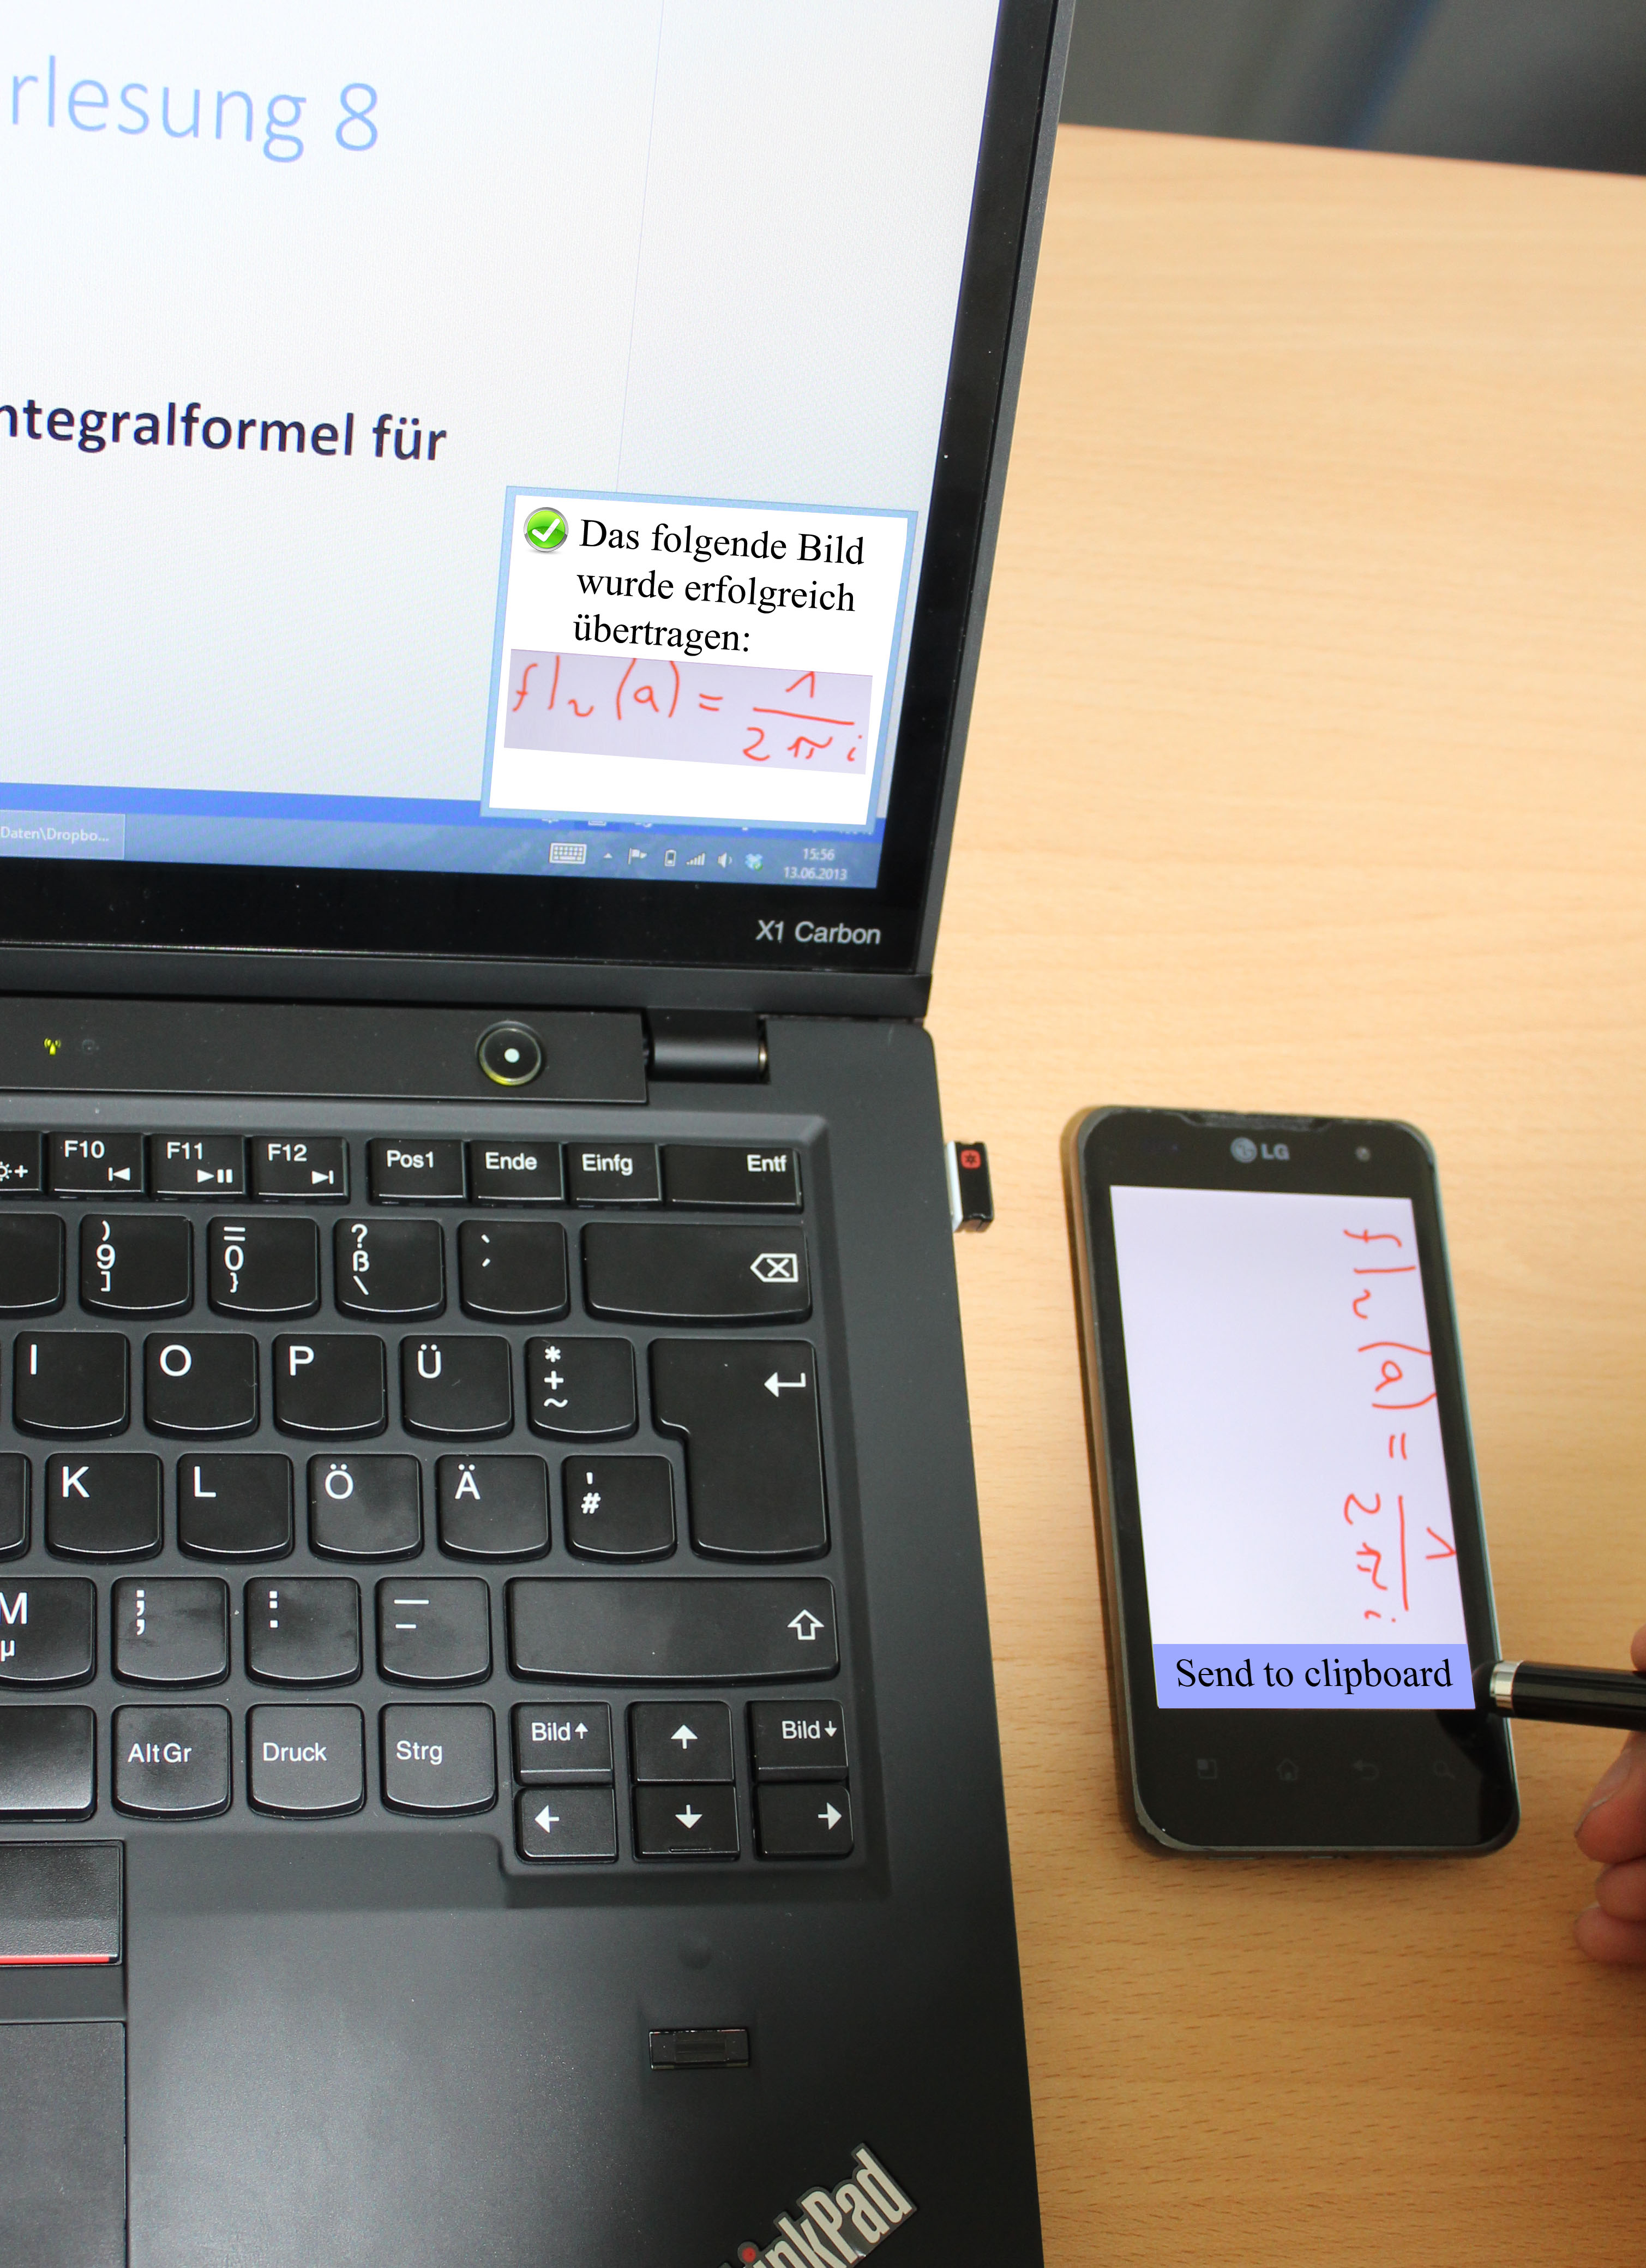
\includegraphics[width=\linewidth]{img/szenario/szenario_3.jpg}
  \caption{Basic user interface (startscreen)}
  \label{fig:mockup_startscreen}
\end{figure}

Am Notebook wird durch einen Hinweis im Tray-Bereich angezeigt, dass Marko die Skizze nun am Notebook bereitgestellt worden ist. Sie ist automatisch in der Zwischenablage des Betriebssystems abgelegt worden, damit Marko die Skizze sofort in seine Notizen einfügen kann. 
Die anderen Studenten im Saal haben natürlich bemerkt, dass Marko die Skizze nun digital verfügbar hat und würden diese auch gerne auf ihrem PC haben. Marko kann nun einfach in der Anwendung am Notebook über das Tray-Icon auswählen, dass er eine Skizze per E-Mail verschicken möchte. Dort gibt es zwei Möglichkeiten, einmal im Standard E-Mail Programm eine vorgefertigte E-Mail zu öffnen, wo die Skizze angehangen ist oder sie direkt an eine vordefinierte Gruppe von Studenten zu verschicken. Marko hat seine Mathe-Lerngruppe schon abgespeichert und kann nun die Skizze direkt per Rundmail an seine Kommilitonen schicken.

% =============================================================================
\section{Low-fidelity Prototyp}
% =============================================================================
In diesem Abschnitt des Papiers wird der low-fidelity Prototyp der Android-Anwendung vorgestellt.\\

Die Startansicht der Anwendung, dargestellt in Abbildung \ref{fig:mockup_startscreen}, zeigt eine am am oberen Bildrand angebrachte Menüleiste, sowie eine große Zeichenfläche mit weißen Hintergrund. 
Die Menüleiste bietet dabei folgenden Funktionen an:

\begin{itemize}
	\item {\textbf{Zeigertool:} Kann verwendet werden um zu zoomen oder die Zeichenfläche nach links, rechts, oben oder unten zu verschieben}
	\item {\textbf{Stift:} Mit dem Stift kann auf der Zeichenfläche gezeichnet werden.}
	\item {\textbf{Farbwahl:} Hier kann eine Stiftfarbe ausgewählt werden}
	\item {\textbf{Stiftdicke:} Hier kann die Dicke des Stiftes ausgewählt werden}
	\item {\textbf{Löschen:} Hier kann die komplette Zeichenfläche geleert werden.}
	\item {\textbf{Senden:} Hier kann die erstellte Zeichnung an das Clipboard des PCs gesendet werden.}
\end{itemize}

\begin{figure}
  \centering
  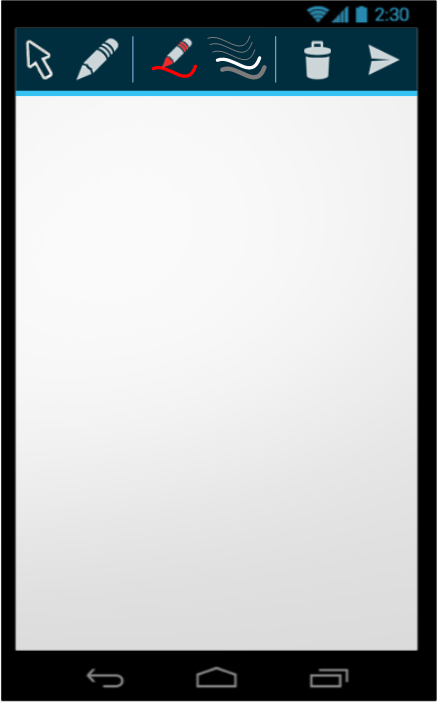
\includegraphics[width=\linewidth]{img/android/mockup_startscreen.png}
  \caption{Basic user interface (startscreen)}
  \label{fig:mockup_startscreen}
\end{figure}

Wird die Funktionaltität "Farbwahl" von Nutzer ausgewählt, erscheint das in Abbildung \ref{fig:mockup_color} dargestellte Auswahlmenü. Die aktuell gewählte Farbe wird dabei sowohl im Auswahlmenü durch eine dicke, weiße Umwandung der Farbe angezeigt, als auch in der Menüliste an der Farbe des Stifts abgebildet.

\begin{figure}
  \centering
  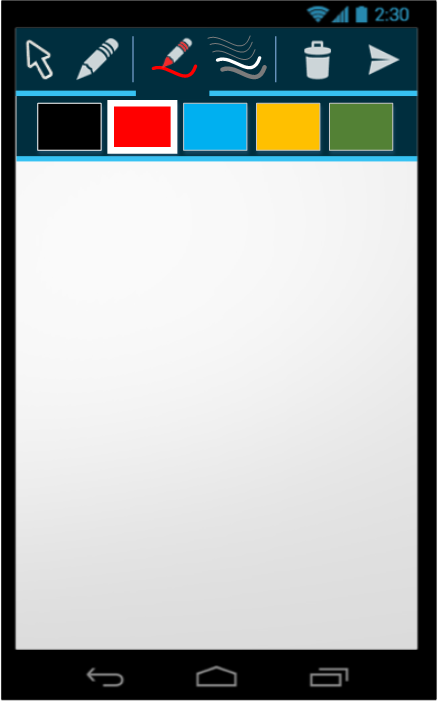
\includegraphics[width=190pt]{img/android/mockup_color.png}
  \caption{Auswahlmenü für die Farbwahl}
  \label{fig:mockup_color}
\end{figure}

Möchte der Nutzer die Dicke des Zeichenstifts verändern, drückt er den im Menü angebrachte Button zur Änderung der Stiftdicke. Darauffolgend erscheint das in Graphik \ref{fig:mockup_pen} abgebildete Auswahlmenü. Die Anzeige der aktuellen Stiftdicke wird analog zur Funktionaltität "Farbwahl" angezeigt.

\begin{figure}
  \centering
  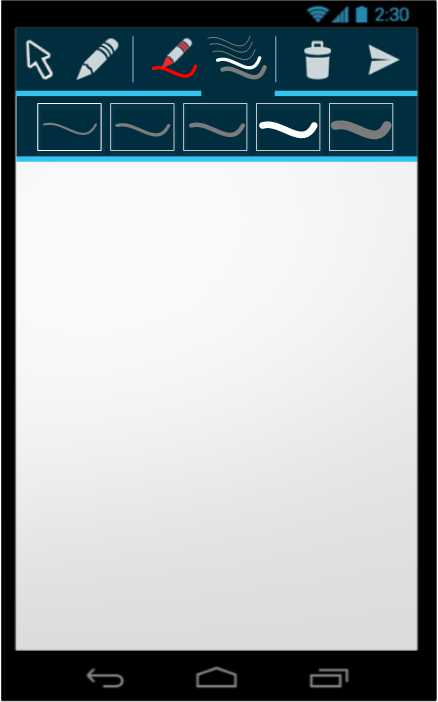
\includegraphics[width=190pt]{img/android/mockup_pen.png}
  \caption{Auswahlmenü für die Stiftdicke}
  \label{fig:mockup_pen}
\end{figure}

% =============================================================================
\section{Ergebnisse der Studie}
% =============================================================================

\subsection{Ziel und Durchführung}
Ziel der Studie war es, Antworten auf die folgenden drei Fragen zu finden:
\begin{itemize}
\item Lässt sich ein Marktpotential der App aus dem aktuellen Notizenverhalten der potentiellen Anwender ableiten?
\item Welche Features sehen diese als unbedingt notwendig an?
\item Welche Gesten würden die Nutzer für die Bedienung der App erwarten und wie bewerten?
\end{itemize}

Die erste Frage sollte dabei klären, dass das Konzept der App auch tatsächlich Probleme der Anwender aufgreift und nicht nur ein Randphänomen adressiert. Anhand der zweiten Frage sollte zudem sicher gestellt werden, dass ein möglichst großer gemeinsamer Nenner hinsichtlich der gewünschten Funktionen erreicht werden würde. Die letzte Frage orientiert sich an der Methode von Wobbrock und sollte eine möglichst intuitive Bedienung der App gewährleisten.

Ein entsprechender Fragebogens wurde (technisch) via Google Forms umgesetzt und den Teilnehmern der Studie via Internet bereitgestellt. Dieser bestand aus drei Hauptteilen:

\begin{itemize}
\item Einordnung des Teilnehmers
\item Vorstellung des Hauptszenarios der App und Gestenerfassung
\item Bewertung des Konzepts der App
\end{itemize}

Der erste Teil enthielt demographische Fragen und sollte dabei helfen, die technische Versiertheit sowie das Notizverhalten des Teilnehmers einzuschätzen.
Der zweite Teil stellte das Hauptszenario unserer App vor und forderte den Teilnehmer dazu auf, drei Gesten zur Bedienung der App in Freitextform anzugeben. Darüber hinaus sollte dieser auch die Anwendbarkeit der angegeben Geste auf einer Skala von 1 (schlecht) bis 5 (gut) bewerten.
Der dritten und letzte Teil enthielt spezifische Fragen zu unserem Konzept; Beispielsweise, ob der Teilnehmer auch tatsächlich Interesse hätte, die App zu verwenden, welche Probleme dieser hinsichtlich der App antizipieren würde oder, wie viel der Teilnehmer für eine solche Anwendung ausgeben würde.

\subsection{Teilnehmer und ihre Eigenschaften}

Insgesamt nahmen 14 Personen an der Studie teil, von denen 13 männlich waren. Das angegebene Alter lag zwischen 22 und 27 und mit einem Mittelwert von 24,36 Jahren (SD = 1,5). Zehn der 14 Teilnehmer gaben einen Informatikstudiengang an. Hinsichtlich ihrer technischen Begeisterung bewerteten sie sich auf einer Skala von 1 (nicht interessiert) bis 5 (sehr interessiert) mit durchschnittlich 4,64 Punkten (SD = 0,5).
Auffallend war auch, dass fast jeder Teilnehmer einen Laptop und ein Smartphone besaß und diese mit zur Universität nahm. Bei Tablets traf dies immerhin auf die Hälfte zu (vgl. Tabelle \ref{fig:studie_tabelle}). Folglich waren die technischen Grundvoraussetzungen für unser Konzept beim Großteil der Teilnehmer gegeben.

\begin{figure}
  \centering
  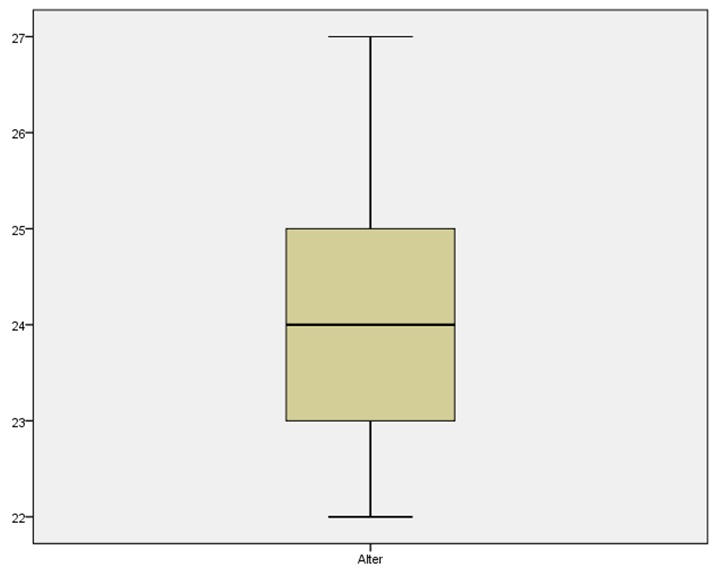
\includegraphics[width=180pt]{img/studie/Alter.jpg}
  \caption{Alter}
  \label{fig:studie_alter}
\end{figure}

\begin{figure}
  \centering
\begin{tabular}{|l|p{1.5cm}|p{3cm}|}
\hline 
 & Gerät vorhanden & Gerät wird zur \newline Uni mitgenommen \\ 
\hline 
Laptop & 14 & 11 \\ 
\hline 
Smartphone & 13 & 12 \\ 
\hline 
Tablet & 7 & 6 \\ 
\hline 
\end{tabular} 
  \caption{Alter}
  \label{fig:studie_tabelle}
\end{figure}

%TODO: Table
Nach diesen eher allgemeinen Einordnungskriterien wurden die Teilnehmer nach ihrem Notizverhalten während eines Meetings, einer Vorlesung oder einer sonstigen Präsentation befragt.
Dabei stellte sich heraus, dass Papier aufgrund seiner zehn Nennungen noch immer das beliebteste Medium zu sein schien. Dazu passend gab auch nur eine Person an, handschriftlichen Aufzeichnungen später zu digitalisieren. Zumindest drei Teilnehmer nutzten auch technische Geräte. Eine Person verzichtete vollständig auf Notizen.
Auf die Frage, warum technische Geräte bisher nicht / selten genutzt würden, antworteten sieben von 14 Personen, dass sie die bestehenden Anwendungen als unzureichend bewerten würden.
Zusammengefasst ergibt sich also, dass die Teilnehmer technischen Geräte mit zur Universität nehmen, aber selten für Notizen nutzen. Außerdem scheinen bisher die richtigen Werkzeuge bzw. Anwendungen zu fehlen, um Laptops und ähnliche Geräte produktiv und komfortabel in den entsprechenden Workflow einbinden zu können.

\subsection{Gestensteuerung}

Als erstes sollten die Teilnehmer eine Geste schildern, durch die sie die Übertragung einer Skizze vom Smartphone an den Computer starten würden (die entsprechende Funktionalität wurde ihnen zuvor gezeigt bzw. erklärt). Sieben der Teilnehmer beschrieben daraufhin eine Wischgeste in Richtung des Laptops. Fünf gaben an, sich für diese Funktionalität keine Geste vorstellen zu können. Hatten die Teilnehmer eine Geste angegeben, so bewerteten sie diese auf einer Skala von 1 (schlechte Geste) bis 5 (gute Geste) mit durchschnittlich 3,86 Punkten (SD = 1,2).

\begin{figure}
  \centering
  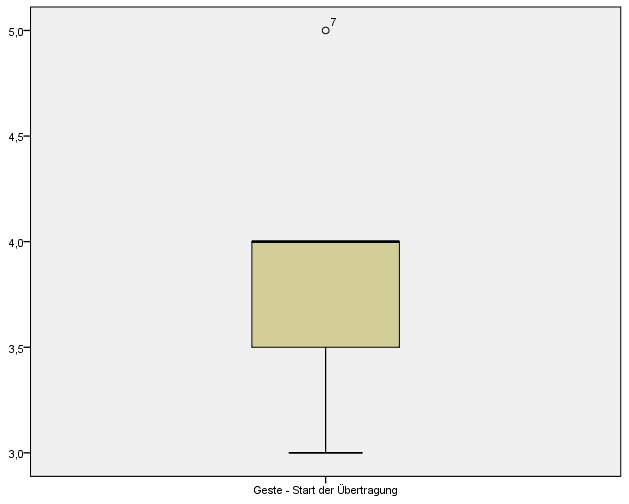
\includegraphics[width=180pt]{img/studie/Geste_Start_Uebertragung.jpg}
  \caption{Geste - Start der Übertragung}
  \label{fig:studie_Geste_Start_Uebertragung}
\end{figure}

\begin{figure}
  \centering
  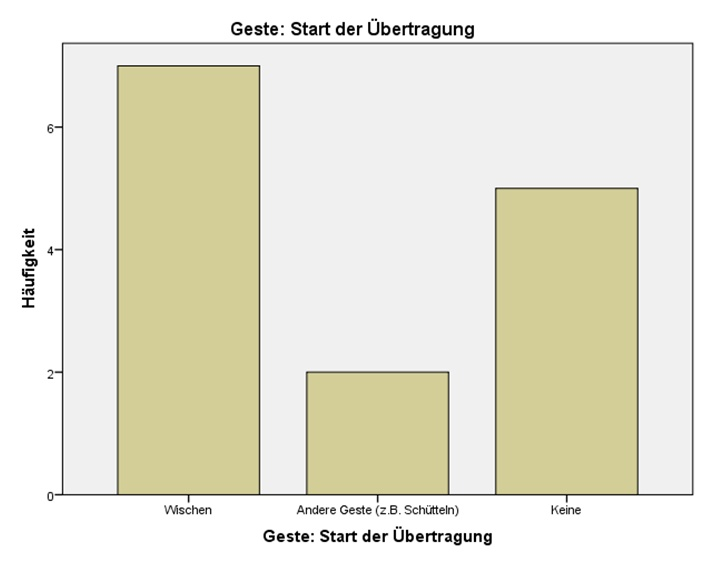
\includegraphics[width=180pt]{img/studie/Antworten_Geste_Start_Uebertragung.jpg}
  \caption{Geste - Start der Übertragung}
  \label{fig:studie_Antworten_Geste_Start_Uebertragung}
\end{figure}


Ein ähnliches Bild ergab die zweite Beschreibung und Auswertung einer Geste, um eine Skizze auf dem Smartphone wiederherzustellen, nachdem sie an den Computer verschickt worden war. Fünf Teilnehmer beschrieben eine Wischgeste in die entgegengesetzte Richtung zu der, die sie zuvor angegeben hatten. Acht gaben nun an, dass ihnen keine Geste eingefallen sei. Die angegebenen Gesten wurden im Durchschnitt mit 3,60 Punkten etwas schlechter bewertet (SD = 0,5).

\begin{figure}
  \centering
  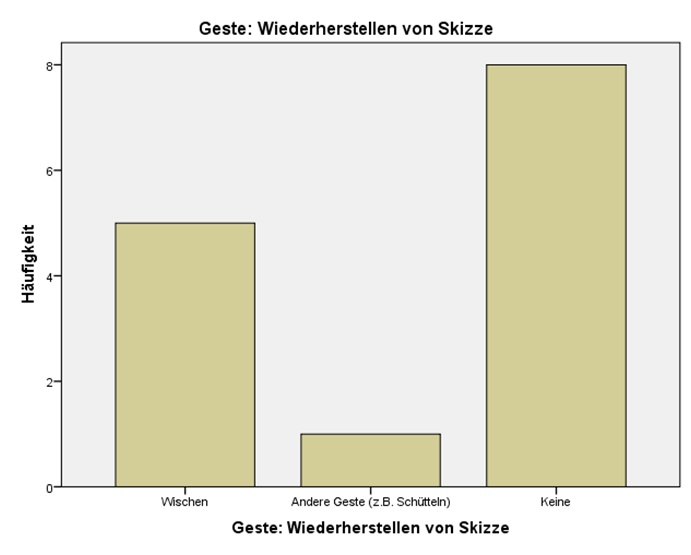
\includegraphics[width=180pt]{img/studie/Antworten_Geste_Wiederherstellen.jpg}
  \caption{Geste - Wiederherstellen von Skizze}
  \label{fig:studie_Antworten_Geste_Wiederherstellen}
\end{figure}


In beiden Fällen schließen wir daraus, dass die Teilnehmer mit ihrer Geste zufrieden, nicht aber “begeistert” waren.
Als drittes wurden die Teilnehmer aufgefordert, eine Geste für die Übertragung der Skizze an mehrere Computer zu beschreiben (Multicast). Hier antworteten nun schon elf Teilnehmer, dass ihnen hierfür keine Geste einfallen würde. Die drei restlichen Gesten waren zudem recht komplex, wie z.B. eine Art Zoomgeste mit fünf Fingern.

\begin{figure}
  \centering
  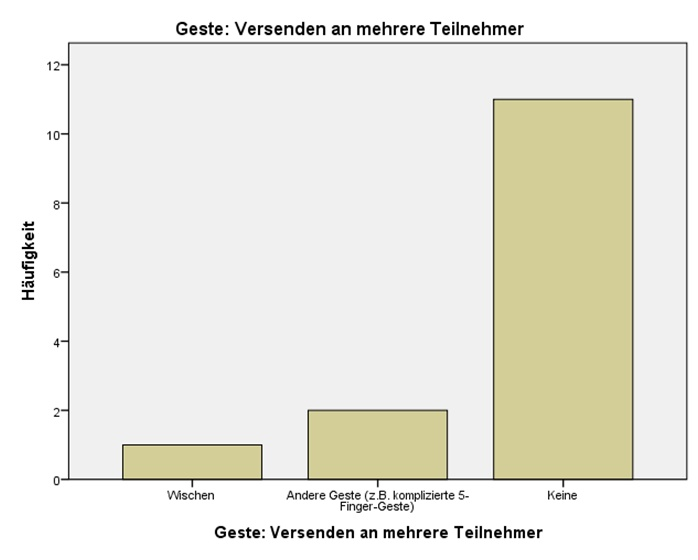
\includegraphics[width=180pt]{img/studie/Antworten_Geste_Multicast.jpg}
  \caption{Geste - Versenden an mehrere Teilnehmer}
  \label{fig:studie_Antworten_Geste_Multicast}
\end{figure}


Auch im Hinblick auf die zuvor angegeben Swipe-Gesten, die mittlerweile doch sehr weit verbreitet sind, liegt daher die Vermutung nahe, dass die Teilnehmer eher in erlernte Bedienszenarien zurückfallen, als wirklich intuitive Gesten zu erwarten bzw. anzuwenden. Auffällig war allerdings, dass die Swipe-Geste immer in Richtung des Laptops erfolgte (in Abhängigkeit von der tatsächlichen Positionierung der beiden Geräte). Da viele, existierende Swipe-Gesten eher statisch ausgeführt werden (z.B. Android-Menübar - top-down), könnte man dies als Beleg dafür anführen, dass die Geste doch intuitiv war. Letztendlich ist hier die Stichprobengröße allerdings zu gering, um eine sinnvolle Aussage treffen zu können.

Als letztes sollten die Teilnehmer angeben, ob sie im Hinblick auf die vorgestellte Anwendung allgemein lieber Menüs oder eine Geste nutzen wollen würden. Auf einer Skala von 1 (Geste) bis 5 (Menü) vergaben dabei 12 von 14 Personen mit 4 oder 5 Punkte, die zwei verbliebenen Teilnehmer allerdings zwei Punkte (M = 4,21, SD = 1,1). 

\begin{figure}
  \centering
  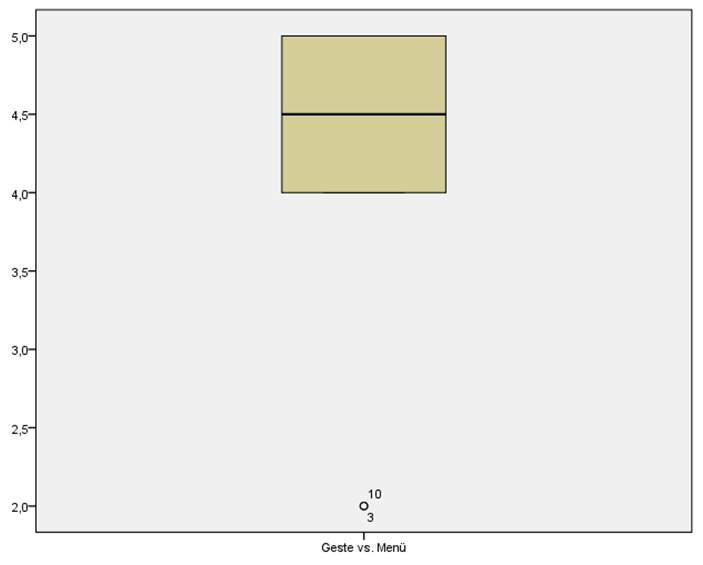
\includegraphics[width=180pt]{img/studie/Geste_vs_Menu.jpg}
  \caption{Geste vs Menü}
  \label{fig:studie_Geste_vs_Menu}
\end{figure}

Folglich scheint eine Menü-basierte Steuerung innerhalb unserer Sichtprobe bevorzugt zu werden. Die beiden “Ausreißer-Bewertungen” lassen jedoch auch die Vermutung zu, dass sich dieses Verhältnis bei einer größeren Stichprobe ändern könnte.

\subsection{Fragen zum Konzept}

Bewertet wurde das Konzept unserer App hauptsächlich anhand der zwei folgenden Fragen:
\begin{enumerate}
\item Wie interessant findest du das Konzept?
\item Würdest du die App verwenden?
\end{enumerate}


Für beide Fragen stand auch hier eine Skala von 1 (uninteressant) bis 5 (interessant) zur Verfügung.
Ihr Interesse an der App bekundeten die Teilnehmer mit durchschnittlich 3,71 Punkten (SD = 0,9). Eine tatsächliche Verwendung der App bewerteten sie im Durchschnitt mit 3,29 Punkten (SD = 1,3), woraus sich eine solide, wenn auch nicht überragend große Nachfrage ableiten ließe.

\begin{figure}
  \centering
  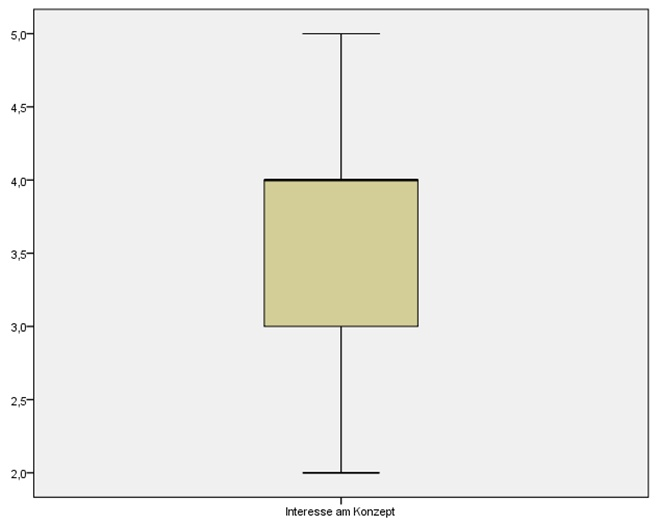
\includegraphics[width=180pt]{img/studie/Interesse_Konzept.jpg}
  \caption{Interesse am Konzept}
  \label{fig:studie_Interesse_Konzept}
\end{figure}

\begin{figure}
  \centering
  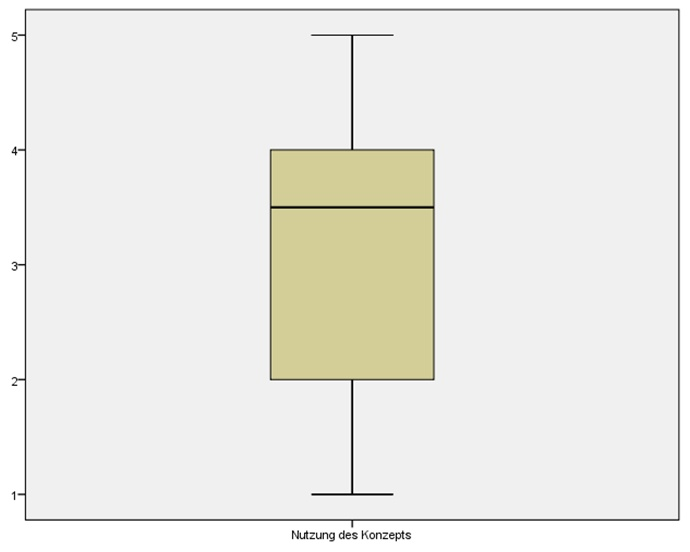
\includegraphics[width=180pt]{img/studie/Nutzung des Konzeptes.jpg}
  \caption{Nutzung des Konzepts}
  \label{fig:studie_Nutzung des Konzeptes}
\end{figure}


Interessant waren in diesem Zusammenhang auch die Antworten auf die Frage nach dem potentiellen Aufwand für eine Erstinstallation. Obwohl oder vielleicht auch gerade weil sich die Nutzer als technisch begeistert einstuften, vergaben die Teilnehmer auf einer Skala von 1 (wenige Minuten) bis 5 (mehrere Stunden) durchschnittlich nur 1,79 Punkte (SD = 1,1).

\begin{figure}
  \centering
  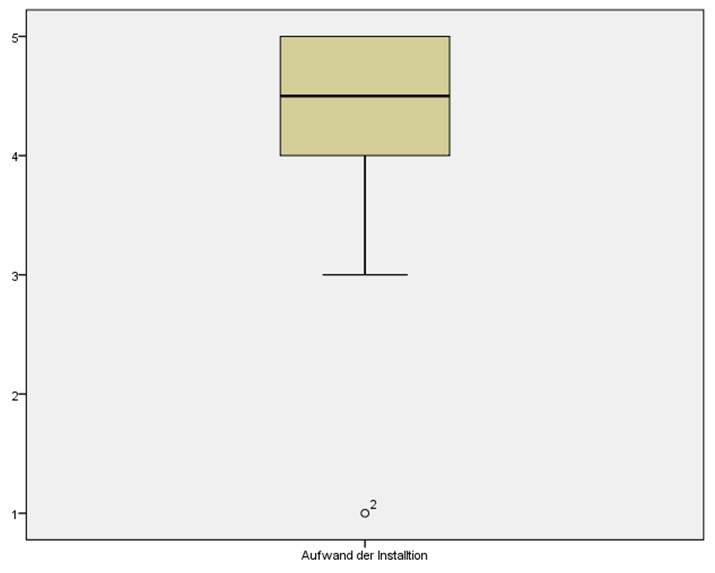
\includegraphics[width=180pt]{img/studie/Aufwand_Installation.jpg}
  \caption{Aufwand der Installation}
  \label{fig:studie_Aufwand_Installation}
\end{figure}

Die Nutzung und den Vorteil eines digitalen Stiftes für die Skizzen auf dem Smartphone und Tablet bewerteten die Teilnehmer weniger überraschend durchweg mit sehr gut. Auf einer Skala von 1 (nicht hilfreich) bis 5 (hilfreich) ergab sich dabei einem Mittelwert von 4,79 Punkten (SD = 0,4). In Folge dessen wäre es wohl sinnvoll, die App in Kombination mit einem entsprechenden Stift anzubieten. Die Teilnehmer der Studie  wären im Mittel 1,95 Euro bereit für die App zu zahlen (SD = 2,8).

\begin{figure}
  \centering
  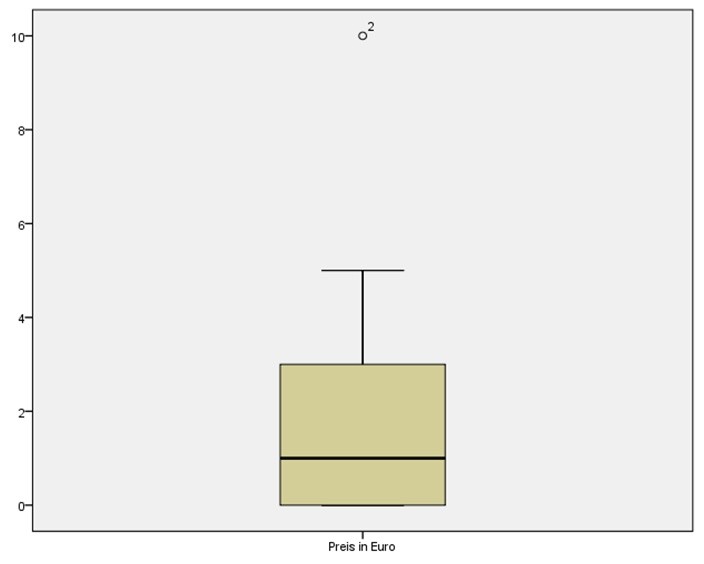
\includegraphics[width=180pt]{img/studie/Preis.jpg}
  \caption{Preis in Euro}
  \label{fig:studie_Preis}
\end{figure}

Zum Schluss gab es zudem noch zwei Freitextfelder für mögliche Probleme und Featurewünsche der Teilnehmer. Bei den möglichen Problemen gab es zwei große Bedenken, nämlich der zu kleine Bildschirm des Smartphones (5 Nennungen) und eine unzureichend genaue Möglichkeit zu zeichnen (4 Nennungen). Demnach könnte sich die Verbreitung von Tablets als relevant erweisen, da diese eine größere Fläche bieten. Wie zuvor erwähnt liegt die Verbreitungsrate innerhalb der Stichprobe hier bei nur ca. 50\%, was sich negativ auf Bewertung und potentielle Nutzung der App auswirken könnte.
Hinsichtlich der gewünschten Features, gab es unzählige Antworten, die zum Teil sehr komplex und wage formuliert waren. So gab ein Teilnehmer beispielsweise an, dass sich die App wie Papier bedienen lasse sollte, man aber alles beliebig rückgängig machen sollte. Daneben kam sogar die Idee auf, die App als bidirektionale Verbindung zwischen Laptop und Smartphone zu realisieren, so dass man über das Smartphone einen vorgegeben Bereich innerhalb eines Dokuments am Computer bearbeiten könnte.


% =============================================================================
\section{Diskussion}
% =============================================================================
Bei der Studie hat sich unter anderem gezeigt, dass, entgegen unserer Erwartungen, die meisten Nutzer für das Auslösen der Übertragung zum Laptop keine Bewegungsgeste mit dem Smartphone sondern eher einen zu betätigenden Button oder eine Wischgeste mit Fingern auf dem Touchscreen des Smartphones bevorzugen. Dies war für uns überraschend, da wir angenommen hatten, dass Bewegungsgesten als natürliche Gesten bevorzugt werden. Jedoch sind Benutzer von Computern an die seit Jahren praktisch überall eingesetzte Maus- und Tastatur-Steuerung gewöhnt, bei der die Bedienung durch das Drücken von Buttons mit der Maus erfolgt. Diese hat sich auch auf Smartphones übertragen, nur werden die Buttons dort per Touchscreen direkt mit dem Finger bedient. Durch diese jahrelange Gewöhnung sehen geübte Benutzer diese Bedienung wohl als völlig natürlich an und empfinden dann daher auch das Betätigen eines Buttons als einfache und benutzerfreundliche Geste. Auch Wischgesten mit den Fingern sind bei der Smartphone-Bedienung heutzutage bereits als natürlich empfunden, wie etwa bei den Standardapps von Google (etwa Google Mail: Liste der Konversationen per seitlicher Wischgeste einblenden oder Menü aufklappen per Wischgeste vom oberen Rand nach unten).
Bewegungsgesten mit dem Smartphone wären damit eher eine Umstellung, auch wenn der Wow-Effekt natürlich größer wäre als beim Betätigen eines Buttons. Für die Weiterentwicklung des Designs ist die Lehre aus diesem Ergebnis jedoch, dass wir dem Benutzer Wahlfreiheit lassen sollten und ihm sowohl die Möglichkeit bieten die Übertragung per Button als auch per Wischgeste anzustoßen. 

Zusätzlich war eine in den Freitextfeldern der Studie oft geäußerte Kritik, dass die Befragten einen Smartphone-Bildschirm als zu klein für Zeichnungen empfinden. Von daher wäre es wichtig, die App auch für Tablets bereitzustellen, oder die Erweiterung der Zeichenfläche über mehrere Smartphone- oder Tabletbildschirme zu implementieren.

Insgesamt lässt sich aber sagen, dass das Konzept von den Befragten positiv bewertet wurde, sodass anzunehmen ist, dass durchaus Marktpotenzial vorhanden ist.


% =============================================================================
\section{Konklusion}
% =============================================================================
In diesem Paper haben wir unser Projekt Copy-To-Clipboard vorgestellt, das wir im Rahmen der HCI-Vorlesung im Sommersemester 2013 an der Universität Augsburg durchgeführt haben. Dabei haben wir die wirkliche Durchführung des Projekts, also die Implementierung außen vor gelassen, und uns auf die HCI-Aspekte des Projekts beschränkt um den iterativen, nutzerzentrierten HCI-Designprozess zu verstehen und anzuwenden.
Der Schwerpunkt lag dabei auf der von uns durchgeführten Studie. Sie diente uns zum Einen dazu, die mögliche Zielgruppe näher kennenzulernen und diese Erkenntnisse in das iterativ erarbeitete Design einzubeziehen. Zum anderen wollten wir, angelehnt an das Verfahren von Wobbrock \cite{Wobbrock}, für das Feature Übertragen der Zeichnung auf den Laptop eine möglichst benutzerfreundliche Geste finden. Auch wenn die Ergebnisse der Studie, insbesondere die favorisierte Geste etwas überraschend waren, so hat es uns im Designprozess gerade deswegen viel weiter geholfen.

Bei einer mehrheitlich von Informatikern beantwortete Studie hat es uns überrascht, dass trotzdem kaum jemand Notizen bereits rein digital anfertigt.
Dies und die Tatsache, dass das Konzept mehrheitlich positiv bewertet wurde, bringt uns zu der Überzeugung, dass sich die Realisierung des Projekts lohnen würde.




\balance
\bibliographystyle{acm-sigchi}
\bibliography{bericht}

\end{document}